\documentclass[12pt]{article}

\usepackage[utf8]{inputenc}
\usepackage[russian]{babel}
\usepackage{geometry}
\usepackage{graphicx}
\usepackage{soul}
\usepackage{color}
\usepackage{colortbl}
\usepackage{amssymb}
\usepackage{multicol}

\setlength{\columnseprule}{0.5pt}
\def\columnseprulecolor{\color{black}}

\geometry{a4paper, top=15mm, bottom=15mm, left=10mm, right=10mm}

\definecolor{cobalt}{RGB}{142, 170, 219}
\definecolor{tacao}{RGB}{244, 176, 131}
\definecolor{feijoa}{RGB}{168, 208, 141}
\definecolor{yellonge}{RGB}{255, 217, 102}


\begin{document}

\setcounter{page}{0}
\thispagestyle{empty}

\begin{center}
    Федеральное государственное автономное учебное учреждение высшего образования\\
    <<Национальный исследовательский университет ИТМО>>\\
\vspace{0.5cm}
    Мегафакультет компьютеных технологий и управления\\
    Факультет программной инженерии и компьютерной техники
\end{center}

\vspace{3cm}

\begin{center}
\Large
\textbf{
    Отчёт\\
    по лабораторной работе №2\\
    <<Синтез помехоустойчивого кода>>\\
    по дисциплине <<Информатика>>
}
\end{center}

\begin{center}
\large
    Вариант 79
\end{center}

\vspace{6cm}

\begin{flushright}
    Студент: Кожухин Иван Алексеевич, группа P3118\\
    Преподаватель: Рыбаков Степан Дмитриевич
\end{flushright}

\vspace{6cm}

\begin{center}
    Санкт-Петербург\\
    2022
\end{center}

\newpage

\tableofcontents

\newpage

\section{Задание}

1. Определить свой вариант задания с помощью номера в ISU (он же номер
студенческого билета). Вариантом является комбинация 3-й и 5-й цифр.
Т. е. если номер в ISU = 123456, то вариант = 35.\\
\\
2. На основании номера варианта задания выбрать набор из 4 полученных
сообщений в виде последовательности 7-символьного кода.\\
\\
3. Построить схему декодирования классического кода Хэмминга (7; 4),
которую представить в отчёте в виде изображения.\\
\\
4. Показать, исходя из выбранных вариантов сообщений (по 4 у каждого –
часть №1 в варианте), имеются ли в принятом сообщении ошибки, и если
имеются, то какие. Подробно прокомментировать и записать правильное
сообщение.\\
\\
5. На основании номера варианта задания выбрать 1 полученное сообщение в
виде последовательности 11-символьного кода.\\
\\
6. Построить схему декодирования классического кода Хэмминга (15; 11),
которую представить в отчёте в виде изображения.\\
\\
7. Показать, исходя из выбранного варианта сообщений (по 1 у каждого –
часть №2 в варианте), имеются ли в принятом сообщении ошибки, и если
имеются, то какие. Подробно прокомментировать и записать правильное
сообщение.\\
\\
8. Сложить номера всех 5 вариантов заданий. Умножить полученное число
на 4. Принять данное число как число информационных разрядов в
передаваемом сообщении. Вычислить для данного числа минимальное
число проверочных разрядов и коэффициент избыточности.\\
\\
9. Необязательное задания для получения оценки <<5>> (позволяет набрать от
86 до 100 процентов от максимального числа баллов БаРС за данную
лабораторную). Написать программу на любом языке программирования,
которая на вход из командной строки получает набор из 7 цифр <<0>> и <<1>>,
записанных подряд, анализирует это сообщение на основе классического
кода Хэмминга (7; 4), а затем выдаёт правильное сообщение (только
информационные биты) и указывает бит с ошибкой при его наличии.

\newpage

\section{Выполнение основного задания}

\begin{figure}[h]
    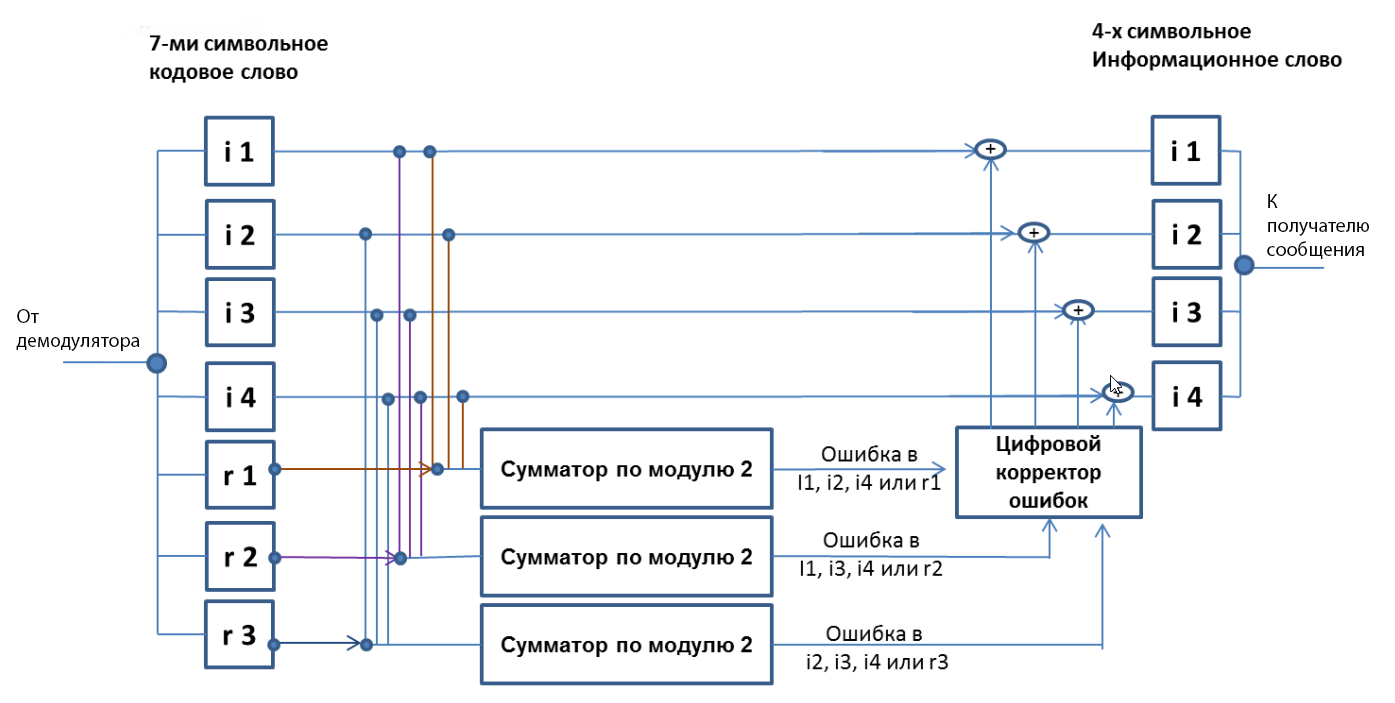
\includegraphics[width=\linewidth]{img/image1.png}
    \caption{Схема декодирования классического кода Хэмминга (7; 4)}
\end{figure}

\subsection{Сообщение №63}

Полученное сообщение: \so{0110100}\\
\\
\begin{tabular}{
|p{1cm}|p{1cm}|p{1cm}|p{1cm}|p{1cm}|p{1cm}|p{1cm}|p{1cm}|p{1cm}|}
    \hline
     & 1 & 2 & 3 & 4 & 5 & 6 & 7 & \\
    \hline
    $2^x$ & $r_1$ & $r_2$ & $i_1$ & $r_3$ & $i_2$ & $i_3$ & $i_4$ & S\\
    \hline
    \textbf{1} & \cellcolor{cobalt} 0 & 1 & \cellcolor{cobalt} 1 & 0 & \cellcolor{cobalt} 1 & 0 & \cellcolor{cobalt} 0 & 0\\
    \hline
    \textbf{2} & 0 & \cellcolor{tacao} 1 & \cellcolor{tacao} 1 & 0 & 1 & \cellcolor{tacao} 0 & \cellcolor{tacao} 0 & 0\\
    \hline
    \textbf{4} & 0 & 1 & 1 & \cellcolor{feijoa} 0 & \cellcolor{feijoa} 1 & \cellcolor{feijoa} 0 & \cellcolor{feijoa} 0 & 0\\
    \hline
\end{tabular}
\\
\\
Решение:\\
1) Определяем синдромы последовательности по формулам:

\begin{multicols}{2}

    \centering

    $S_1 = r_1 \oplus i_1 \oplus i_2 \oplus i_4$\\
    $S_2 = r_2 \oplus i_1 \oplus i_3 \oplus i_4$\\
    $S_2 = r_3 \oplus i_2 \oplus i_3 \oplus i_4$\\
    
    \columnbreak

    $S_1 = 0 \oplus 1 \oplus 1 \oplus 0 = 0$\\
    $S_2 = 1 \oplus 1 \oplus 0 \oplus 0 = 0$\\
    $S_2 = 0 \oplus 1 \oplus 0 \oplus 0 = 1$\\

\end{multicols}

\noindent 2) Получаем последовательность синдромов: \so{001}\\
3) Переводим $100_2 = 4_{10}$, $\Rightarrow$ ошибка в бите №4\\
4) Меняем бит №4 на обратный\\
5) Получаем правильное сообщение: \so{0111100}

\newpage

\subsection{Сообщение №35}

Полученное сообщение: \so{0111010}\\
\\
\begin{tabular}{
|p{1cm}|p{1cm}|p{1cm}|p{1cm}|p{1cm}|p{1cm}|p{1cm}|p{1cm}|p{1cm}|}
    \hline
     & 1 & 2 & 3 & 4 & 5 & 6 & 7 & \\
    \hline
    $2^x$ & $r_1$ & $r_2$ & $i_1$ & $r_3$ & $i_2$ & $i_3$ & $i_4$ & S\\
    \hline
    \textbf{1} & \cellcolor{cobalt} 0 & 1 & \cellcolor{cobalt} 1 & 1 & \cellcolor{cobalt} 0 & 1 & \cellcolor{cobalt} 0 & 1\\
    \hline
    \textbf{2} & 0 & \cellcolor{tacao} 1 & \cellcolor{tacao} 1 & 1 & 0 & \cellcolor{tacao} 1 & \cellcolor{tacao} 0 & 1\\
    \hline
    \textbf{4} & 0 & 1 & 1 & \cellcolor{feijoa} 1 & \cellcolor{feijoa} 0 & \cellcolor{feijoa} 1 & \cellcolor{feijoa} 0 & 0\\
    \hline
\end{tabular}
\\
\\
Решение:\\
1) Определяем синдромы последовательности по формулам:

\begin{multicols}{2}

    \centering

    $S_1 = r_1 \oplus i_1 \oplus i_2 \oplus i_4$\\
    $S_2 = r_2 \oplus i_1 \oplus i_3 \oplus i_4$\\
    $S_2 = r_3 \oplus i_2 \oplus i_3 \oplus i_4$\\

    \columnbreak

    $S_1 = 0 \oplus 1 \oplus 0 \oplus 0 = 1$\\
    $S_2 = 1 \oplus 1 \oplus 1 \oplus 0 = 1$\\
    $S_2 = 1 \oplus 0 \oplus 1 \oplus 0 = 0$\\

\end{multicols}

\noindent 2) Получаем последовательность синдромов: \so{110}\\
3) Переводим $011_2 = 3_{10}$, $\Rightarrow$ ошибка в бите №3\\
4) Меняем бит №3 на обратный\\
5) Получаем правильное сообщение: \so{0101010}

\subsection{Сообщение №75}

Полученное сообщение: \so{0101101}\\
\\
\begin{tabular}{
|p{1cm}|p{1cm}|p{1cm}|p{1cm}|p{1cm}|p{1cm}|p{1cm}|p{1cm}|p{1cm}|}
    \hline
     & 1 & 2 & 3 & 4 & 5 & 6 & 7 & \\
    \hline
    $2^x$ & $r_1$ & $r_2$ & $i_1$ & $r_3$ & $i_2$ & $i_3$ & $i_4$ & S\\
    \hline
    \textbf{1} & \cellcolor{cobalt} 0 & 1 & \cellcolor{cobalt} 0 & 1 & \cellcolor{cobalt} 1 & 0 & \cellcolor{cobalt} 1 & 0\\
    \hline
    \textbf{2} & 0 & \cellcolor{tacao} 1 & \cellcolor{tacao} 0 & 1 & 1 & \cellcolor{tacao} 0 & \cellcolor{tacao} 1 & 0\\
    \hline
    \textbf{4} & 0 & 1 & 0 & \cellcolor{feijoa} 1 & \cellcolor{feijoa} 1 & \cellcolor{feijoa} 0 & \cellcolor{feijoa} 1 & 1\\
    \hline
\end{tabular}
\\
\\
Решение:\\
1) Определяем синдромы последовательности по формулам:

\begin{multicols}{2}


    $S_1 = r_1 \oplus i_1 \oplus i_2 \oplus i_4$\\
    $S_2 = r_2 \oplus i_1 \oplus i_3 \oplus i_4$\\
    $S_2 = r_3 \oplus i_2 \oplus i_3 \oplus i_4$\\

    \columnbreak

    $S_1 = 0 \oplus 0 \oplus 1 \oplus 1 = 0$\\
    $S_2 = 1 \oplus 0 \oplus 0 \oplus 1 = 0$\\
    $S_2 = 1 \oplus 1 \oplus 0 \oplus 1 = 1$\\

\end{multicols}

\noindent 2) Получаем последовательность синдромов: \so{001}\\
3) Переводим $100_2 = 4_{10}$, $\Rightarrow$ ошибка в бите №4\\
4) Меняем бит №4 на обратный\\
5) Получаем правильное сообщение: \so{0100101}

\newpage

\begin{figure}[h]
    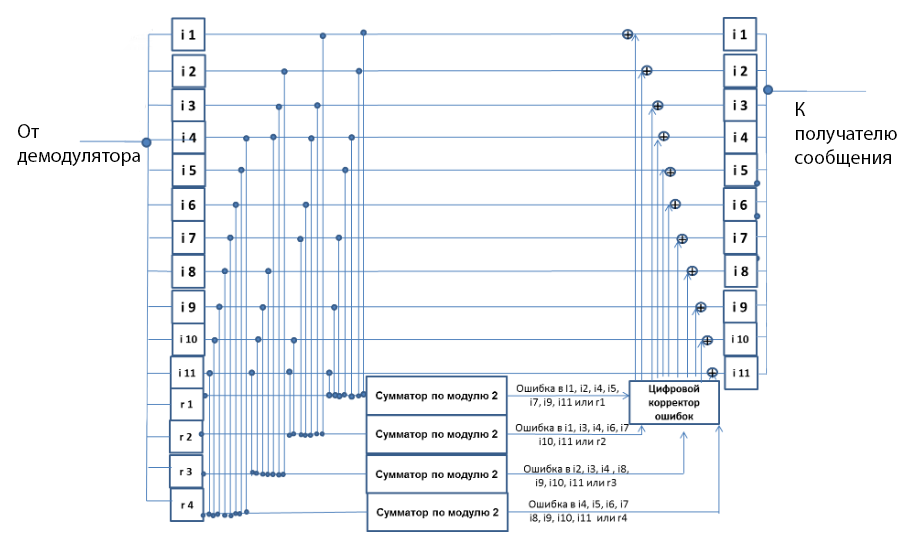
\includegraphics[width=\linewidth]{img/image2.png}
    \caption{Схема декодирования классического кода Хэмминга (15; 11)}
\end{figure}

\subsection{Сообщение №78 (15; 11)}

Полученное сообщение: \so{001110011100100}\\
\\
\begin{tabular}{
|c|c|c|c|c|c|c|c|c|c|c|c|c|c|c|c|c|}
    \hline
     & 1 & 2 & 3 & 4 & 5 & 6 & 7 & 8 & 9 & 10 & 11 & 12 & 13 & 14 & 15 & \\
    \hline
    $2^x$ & $r_1$ & $r_2$ & $i_1$ & $r_3$ & $i_2$ & $i_3$ & $i_4$ & $r_4$ & $i_5$ & $i_6$ & $i_7$ &
    $i_8$ & $i_9$ & $i_{10}$ & $i_{11}$ & S\\
    \hline
    \textbf{1} & \cellcolor{cobalt} 0 & 0 & \cellcolor{cobalt} 1 & 1 & \cellcolor{cobalt} 1 & 0 & \cellcolor{cobalt} 0 & 1 & \cellcolor{cobalt} 1 & 1 & \cellcolor{cobalt} 0 & 0 & \cellcolor{cobalt} 1 & 0 & \cellcolor{cobalt} 0 & 0\\
    \hline
    \textbf{2} & 0 & \cellcolor{tacao} 0 & \cellcolor{tacao} 1 & 1 & 1 & \cellcolor{tacao} 0 & \cellcolor{tacao} 0 & 1 & 1 & \cellcolor{tacao} 1 & \cellcolor{tacao} 0 & 0 & 1 & \cellcolor{tacao} 0 & \cellcolor{tacao} 0 & 0\\
    \hline
    \textbf{4} & 0 & 0 & 1 & \cellcolor{feijoa} 1 & \cellcolor{feijoa} 1 & \cellcolor{feijoa} 0 & \cellcolor{feijoa} 0 & 1 & 1 & 1 & 0 &
    \cellcolor{feijoa} 0 & \cellcolor{feijoa} 1 & \cellcolor{feijoa} 0 & \cellcolor{feijoa} 0 & 1\\
    \hline
    \textbf{8} & 0 & 0 & 1 & 1 & 1 & 0 & 0 & \cellcolor{yellonge} 1 & \cellcolor{yellonge} 1 & \cellcolor{yellonge} 1 & \cellcolor{yellonge} 0 & \cellcolor{yellonge} 0 & \cellcolor{yellonge} 1 & \cellcolor{yellonge} 0 & \cellcolor{yellonge} 0 & 0\\
    \hline
\end{tabular}
\\
\\
Решение:\\
1) Определяем синдромы последовательности по формулам:

\begin{multicols}{2}

    \centering

    $S_1 = r_1 \oplus i_1 \oplus i_2 \oplus i_4 \oplus i_5 \oplus i_7 \oplus i_9 \oplus i_{11}$\\
    $S_2 = r_2 \oplus i_1 \oplus i_3 \oplus i_4 \oplus i_6 \oplus i_7 \oplus i_{10} \oplus i_{11}$\\
    $S_3 = r_3 \oplus i_2 \oplus i_3 \oplus i_4 \oplus i_8 \oplus i_9 \oplus i_{10} \oplus i_{11}$\\
    $S_4 = r_4 \oplus i_5 \oplus i_6 \oplus i_7 \oplus i_8 \oplus i_9 \oplus i_{10} \oplus i_{11}$\\

    \columnbreak

    $S_1 = 0 \oplus 1 \oplus 1 \oplus 0 \oplus 1 \oplus 0 \oplus 1 \oplus 0 = 0$\\
    $S_2 = 0 \oplus 1 \oplus 0 \oplus 0 \oplus 1 \oplus 0 \oplus 0 \oplus 0 = 0$\\
    $S_3 = 1 \oplus 1 \oplus 0 \oplus 0 \oplus 0 \oplus 1 \oplus 0 \oplus 0 = 1$\\
    $S_4 = 1 \oplus 1 \oplus 1 \oplus 0 \oplus 0 \oplus 1 \oplus 0 \oplus 0 = 0$\\

\end{multicols}

\noindent 2) Получаем последовательность синдромов: \so{0010}\\
3) Переводим $0100_2 = 4_{10}$, $\Rightarrow$ ошибка в бите №4\\
4) Меняем бит №4 на обратный\\
5) Получаем правильное сообщение: \so{001010011100100}

\newpage

\subsection{Арифметические вычисления}

$(63 + 10 45 + 75 + 78) \times 4 = 1044$\\
По формуле минимального числа контрольных разрядов:\\
$2^r \ge r + 1065$, отсюда $r = 11$.\\
Коэффициент избыточности:\\
$$\frac{r}{n} = \frac{r}{i + r} = \frac{11}{1055} \approx 0,0104$$

\section{Выполнение дополнительного задания}

\subsection{Код программы на языке Python}
\begin{verbatim}
    message = str(input())
    
    try:
        check = int(message, 2)
    except:
        print('Wrong input format, please enter a binary sequence')
    else:
        syndrome1 = str((int(message[0]) + int(message[2])
                         + int(message[4]) + int(message[6])) % 2)
        syndrome2 = str((int(message[1]) + int(message[2])
                         + int(message[5]) + int(message[6])) % 2)
        syndrome3 = str((int(message[3]) + int(message[4])
                         + int(message[5]) + int(message[6])) % 2)
                         
        errorBit = int(syndrome3 + syndrome2 + syndrome1, 2)
        if errorBit == 0:
            fixedMessage = message
            print('No error')
            print(f'The correct message is {fixedMessage}')
            print(f'The correct info bits are {fixedMessage[2] + fixedMessage[4]
                                               + fixedMessage[5] + fixedMessage[6]}')
        else:
            print(f'Bit #{errorBit} is wrong')
            fixedMessage = ''
            for i in range(len(message)):
                if i == errorBit - 1:
                    fixedMessage += str((int(message[i]) + 1) % 2)
                else:
                    fixedMessage += message[i]
            print(f'The correct message is {fixedMessage}')
            print(f'The correct info bits are {fixedMessage[2] + fixedMessage[4]
                                               + fixedMessage[5] + fixedMessage[6]}')
\end{verbatim}

\newpage

\subsection{Вывод программы}

\begin{figure}[h]
    \centering
    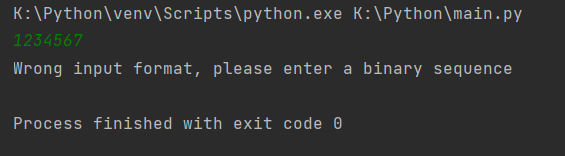
\includegraphics[width=0.92\linewidth]{img/image4.png}
    \caption{Результат работы программы при попытке ввести десятичное число}
\end{figure}

\begin{figure}[h]
    \centering
    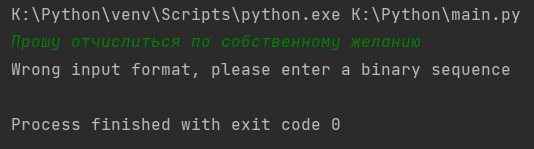
\includegraphics[width=0.92\linewidth]{img/image5.png}
    \caption{Результат работы программы при попытке ввести текст}
\end{figure}

\begin{figure}[h]
    \centering
    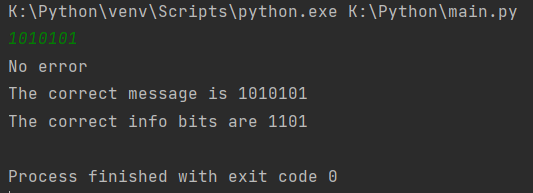
\includegraphics[width=0.92\linewidth]{img/image6.png}
    \caption{Результат работы программы при отсутствии ошибки в сообщении}
\end{figure}

\newpage

\begin{figure}[h]
    \centering
    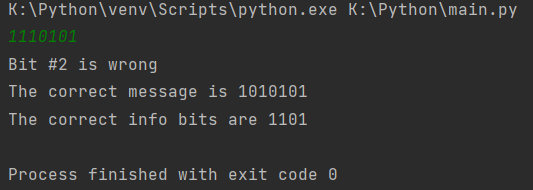
\includegraphics[width=0.92\linewidth]{img/image7.png}
    \caption{Результат работы программы при наличии ошибки в сообщении}
\end{figure}

\newpage

\section{Вывод}

В ходе работы над лабораторной работой я научился декодировать сообщения с помощью классического кода Хэмминга, искать ошибки в переданных сообщениях и исправлять их, рассчитывать минимальное число проверочных разрядов для определенного количества информационных разрядов и коэффициент избыточности сообщения. Также я попрактиковался в программировании на языке Python в ходе выполнения дополнительного задания.

\section{Список использованной литературы}

1. Балакшин П. В. Информатика: лабораторные работы и тесты / П.В. Балакшин, В.В. Соснин, И.В. Калинин, Т.А. Малышева, С.В. Раков, Н.Г. Рущенко, А.М. Дергачев – СПб.: Университет ИТМО, 2019.- 59 с.\\
2. Форум StackOverflow [электронный ресурс]. – Режим доступа: https://ru.stackoverflow.com/ (дата обращения: 17.10.2022)

\end{document}